\documentclass{article}
% ============================================================================
% Aligned but Apart -- TMLR submission build (double-blind).
% Requires tmlr.sty (from https://github.com/mlresearch/tmlr-style or the TMLR
% author kit). Compile: latexmk -pdf main.tex   (or upload to Overleaf).
% Shared content lives at paper/sections, paper/figures, paper/references.bib
% and is reached through ../../ ; this file holds only venue furniture.
% ============================================================================
\usepackage{tmlr}                 % TMLR style; use \usepackage[accepted]{tmlr} for camera-ready
\usepackage{graphicx}
\graphicspath{{../../}}
\usepackage{booktabs}
\usepackage{amsmath,amssymb}
\usepackage{siunitx}
\usepackage{xcolor}
\usepackage[most]{tcolorbox}
\usepackage[hidelinks]{hyperref}

\title{Aligned but Apart: Why Cosine Conflict Diagnostics\\
Misread Auxiliary-Loss Interference at the Output Projection}

% Single author: fill in identifying details for camera-ready.
\author{\name Author Name \email author@institution.edu \\
  \addr Institution}

\def\month{07}
\def\year{2026}
\def\openreview{\url{https://openreview.net/forum?id=XXXXXXXXXX}}

% Anonymized code link. TMLR submission is double-blind: this must point at an
% anonymous mirror (e.g. anonymous.4open.science), NOT a personal GitHub URL.
% Replace the placeholder before upload; the accepted build swaps in the real URL.
\newcommand{\repourl}{\texttt{[[ TODO BEFORE SUBMISSION: anonymized repository URL ]]}}

\begin{document}
\maketitle

\begin{abstract}
Cosine similarity between task gradients is the standard instrument for detecting
\emph{conflict} in auxiliary-loss training: a negative cosine reads as
interference, and gradient surgery acts on it. At a language model's shared,
tied output projection it is misleading. We measure the per-row gradients a
next-token (CE) and an auxiliary multi-token (MTP) loss deposit there, and find
them aligned in direction. On the ${\approx}8\%$ of rows that receive a target
the median per-row cosine is ${\approx}0.53$ and only ${\approx}3$--$4\%$ are
opposed; the remaining ${\approx}92\%$ are scalar multiples, cosine $+1$ by
construction. The tensor is \emph{tied}, so an embedding-path contribution to
those cosines is unbounded here (Sections~\ref{sec:instrument},~\ref{sec:limitations}).
Yet the \emph{aggregate} cosine runs from ${-}0.08$ to ${-}0.19$ under Muon,
shallow enough at one end to read as benign, and ${-}0.28$ to ${-}0.34$ under
AdamW. What comes apart is the two readings, not the supports: per-row gradient
\emph{norms} (three seeds, both optimizers) put both losses on the \emph{same}
rows, at a norm-profile cosine of $0.98$, but $60$--$69\%$ of that mass sits on
${\approx}0.3\%$ of rows, the most frequent function words and punctuation. This
is norm-weighted cancellation, not disjoint support.
An exact rewrite shows the shared-head objective is cross-entropy toward a
next-and-future-token mixture, whose zero-parameter KL cost reproduces
$62$--$91\%$ of the matched within-sweep gap across estimator variants. That
makes the shifted optimum, not gradient conflict, the leading account of the
$+0.39$-nat degradation we measure at 124M ($p{\approx}8{\times}10^{-5}$). Here
the aggregate cosine is \emph{uninformative about where interference lives}.
\end{abstract}



\section{Introduction}
\label{sec:intro}

Predicting several future tokens at once (multi-token prediction, MTP) has
become a common ingredient in large-scale language modeling, used to improve
sample efficiency and to enable self-speculative decoding
\citep{gloeckle2024mtp,deepseekv3}. The auxiliary objective is double-edged: a
growing body of work reports that adding it can \emph{degrade} the primary
next-token objective, particularly at smaller scales and longer horizons
\citep{gloeckle2024mtp,zuhri2025top}. Asked why, practitioners reach for the
intuition that pervades multi-task learning: the two losses must pull the shared
parameters in \emph{conflicting directions}, and the remedy is to detect and
neutralize that conflict, typically from the sign of a gradient cosine
\citep{yu2020pcgrad,wang2021gradvaccine}. This intuition has been questioned in
auxiliary-task learning: \citet{jiang2023forkmerge} report that gradient-conflict
coordination can overlook auxiliary-target generalization, so the cosine signal
does not by itself determine negative transfer. We ask what that signal actually
measures at a language model's shared output head.

This paper is a measurement study of that intuition for the case of an auxiliary
multi-token objective sharing a model's tied output projection. Our central
finding is diagnostic: \textbf{the cosine conflict signal is misleading here.} We
instrument the gradient each loss deposits on the output projection and examine
it \textbf{row by row} (one row per vocabulary item). Two facts emerge, both from
data already in hand. First, the per-row gradients are not opposed; they are \emph{aligned}. We measure this on the rows that receive a target in the measurement batch, the ${\approx}8\%$ that are not scalar multiples by construction (Section~\ref{sec:aligned}). On those rows the median per-row cosine is ${\approx}0.53$, and ${\approx}3$--$4\%$ are opposed. Over all rows the median is $+1$ and $98.4\%$ have $|\cos| > 0.3$. On the matched active-row denominator, $83\%$ of active rows have $\cos > 0.3$; a control that measures CE against an unrelated L1 loss on the same rows reads $1.0\%$. Either way the per-row directions are
predominantly aligned, in sharp contrast to the near-zero aggregate. Second,
the \emph{aggregate} cosine over the flattened matrix is nonetheless near zero,
and tracking it over training shows the two metrics \textbf{start together} (both
$\approx +0.99$ at initialization) and then \textbf{decouple}: within ${\sim}200$
steps the aggregate falls below zero while the per-row median stays at
$\approx +1$. By count, almost no rows are opposed. But the aggregate cosine is magnitude-weighted, so we instrumented the per-row gradient norms directly to see where the weight lies. The two losses load their magnitude on the \emph{same} rows: the norm-profile cosine, meaning the cosine of the two per-row norm vectors, is $0.98$. Yet a tiny high-norm opposed minority, ${\approx}0.3\%$ of rows, carries $60$--$69\%$ of the mass across optimizers. It is this minority that pulls the flattened sum negative. The
alignment is real and holds for the vast majority of rows; the aggregate is a
\emph{norm-weighted cancellation} the cosine cannot localize.

We frame this norm-weighted opposition as the structure a cosine diagnostic
cannot see (Figure~\ref{fig:schematic}), and we relate it to the observed
degradation without claiming to have isolated its cause. Adding the shared MTP objective degrades next-token loss by
${\approx}0.39$ nats (${\approx}10\%$) at 124M, a large and unambiguous effect
(Welch's unequal-variance $t$-test, $p\approx 8\times10^{-5}$), yet it co-occurs with aligned, not
conflicting, per-row gradients (the degradation is measured on the full
30{,}517-step run; per-row alignment on the diagnostic runs above). Three further
observations, all from committed
runs, are consistent with a norm-weighting/capacity account rather than a
directional-conflict one. (i) Conflict-targeted gradient surgery does not recover
the baseline even though the opposition it targets is real and mass-dominant: the
opposed rows are negligible by count ($0.3\%$) but carry the majority of the
gradient-magnitude mass ($60$--$69\%$), and per-row Gram--Schmidt on the head
(Appendix~\ref{app:surgery}) removes exactly that opposition, yet the degradation
does not move. The opposition the aggregate cosine detects is mass-dominant and causally inert (single-seed; Appendix~\ref{app:surgery}). (ii) Detaching the auxiliary's gradient from
the shared head makes the damage \emph{worse}, not better. The probe forms the
auxiliary logits as $\mathrm{sg}(W)h$, so the auxiliary still trains the trunk and
only the head's auxiliary gradient is removed; it is confounded because the head can
no longer co-adapt to the representations the auxiliary shapes, and we treat it as
suggestive only. (iii)
An auxiliary that avoids the shared head (a layer-split contrastive auxiliary)
reduces but does \emph{not} eliminate the gap. These auxiliaries change the objective
as well as its capacity, so the capacity ingredient is not isolated; the untested comparison that would isolate it is separate-head MTP (Section~\ref{sec:limitations}). The figures above are for the contrastive auxiliary: its standard variant is demonstrably short of the CE-only baseline ($\Delta{+}0.039$, $p \approx 0.010$), while a hyperparameter-tuned variant sits below our detection floor, the smallest difference these seed counts can resolve ($\Delta{+}0.018$, $p \approx 0.19$), and is inconclusive. We rest the capacity conclusion on the standard variant.

An exact rewrite of the shared-head objective ties these three observations
together. The objective is cross-entropy against a next-and-future-token mixture label, in effect label smoothing toward the future (an analogy: conventional label smoothing mixes toward the uniform distribution, whereas this mixes toward future-token targets). Its minimizer is therefore not the next-token distribution, which makes the degradation a plausible cost of the target rather than of the optimization path. On that reading
the norm-weighting/capacity observations are subsumed rather than displaced: surgery
would be inert because reprojecting gradients does not move an optimum (i; exact for symmetric projection, empirical for our head-only variants, Section~\ref{sec:discussion}), and
separating capacity would help because it stops the two objectives from sharing one
label (iii). A zero-parameter estimate of the implied KL cost accounts, raw,
for $62$--$91\%$ of the matched within-sweep gap ($0.3715$) across estimator
variants; the coverage-extrapolated full-mixture variant lands at ${\approx}88$--$89\%$, leaving a residual we name
rather than assign.

These findings carry a methodological point beyond MTP. Cosine-based conflict
detection is standard practice in multi-task and auxiliary-learning optimization
\citep{yu2020pcgrad,wang2021gradvaccine,du2018auxsim}, and it is the wrong
instrument in this regime, misleading in two opposite directions depending on the
optimizer. Under Muon the head aggregate sits near zero (${-}0.08$ to ${-}0.19$
across measurement batches), which a practitioner treating near-zero as benign reads
as ``no interference'' while the loss degrades regardless. Under AdamW it goes
negative enough to trip a conflict flag, yet surgery targeting exactly that
opposition recovers nothing. Both readings are of the \emph{head} aggregate; a
practitioner applying a strict sign rule, or aggregating over all parameters, would
flag conflict under both optimizers (Section~\ref{sec:general}). The
decomposition that exposes the problem separates \textbf{direction} (cosine) from
\textbf{support} (where each gradient's magnitude lives). Two additional
measurements sharpen the picture and guard against over-reading it. The high
per-row alignment is \textbf{general} across the network's weight matrices (attention and MLP matrices show it too, many with strongly \emph{negative}
aggregate cosine), so the output head is not special because the metric singles
it out; it is consequential because it directly produces the logits. And the
alignment \textbf{persists when the head is untied}, so it is a property of the
output-projection gradient, not an artifact of weight tying. A full-vocabulary
reading suggests rarer tokens align more, but we show this is a construction
artifact: rare tokens are almost never active, so their rows are dominated by
the cosine-$+1$ parallel majority, and on active rows the effect vanishes. Finally,
our account is a direction-space, multi-loss
complement to \citet{godey2026lmhead}, who show that backpropagating a
\emph{single} loss through the low-rank output head destroys most of its gradient
\emph{norm}; we ask what a \emph{cosine} diagnostic reports when \emph{two} losses
share that head, and answer that their per-row directions align while a high-norm
opposed minority sets the aggregate: measured directly via the per-row gradient
norms (Section~\ref{sec:mechanism}), not inferred.

We are explicit about scope. Every result is for a \textbf{single shared tied
output head}, at 124M ($n{=}5$) and 350M (single seed), undertrained, small-batch.
We do \emph{not} claim that multi-token prediction \emph{as practiced} (separate per-horizon
heads or modules, typically feeding a shared unembedding) degrades next-token modeling; establishing that would require a
separate-head experiment we identify as the primary future step (Section~\ref{sec:limitations}), along with $n{=}3$ at 350M and matched-seed
surgery. What we do establish, on data in hand, is that the standard cosine
conflict diagnostic misreads this regime, and why.

\paragraph{Contributions.} All on a controlled, reproducible GPT-2 testbed (124M
primary, 350M illustrative; FineWeb-Edu) with open code and a committed statistics
script:
\begin{itemize}
\item \textbf{A diagnostic result (Figures~\ref{fig:perrow},~\ref{fig:emergent}).}
  For an auxiliary multi-token objective sharing the tied output projection, the
  per-row gradients of the two losses are \emph{aligned in direction} on the rows
  that carry a target (active-row median cosine ${\approx}0.53$, ${\approx}3$--$4\%$
  opposed; over the full vocabulary the median is $+1$ because ${\approx}92\%$
  of rows are scalar multiples by construction), while the aggregate cosine is
  $\approx 0$, and this decoupling \emph{emerges during training} from an aligned
  start. Standard cosine-based conflict diagnostics therefore \emph{misdiagnose}
  this regime.
\item \textbf{A norm decomposition of the collapse, and a direct measurement of
  its cause (Figures~\ref{fig:normsupport},~\ref{fig:normdecomp}).} Via an exact
  identity, the aggregate would read $+0.94$/$+0.96$ if gradient magnitude were
  flat across rows but reads $-0.08$/$-0.28$: the collapse is set by per-row
  \emph{norm} structure, not by the typical per-row direction. Instrumenting the per-row norms directly (\texttt{measure\_norm\_support.py}; $n{=}3$ seeds per optimizer) settles which structure. The two losses load the \emph{same} rows: norm-profile cosine $0.98$. A high-norm opposed minority carries the majority of the mass: opposed-norm fraction $0.60$ under Muon and $0.69$ under AdamW. The
  aggregate is a norm-weighted cancellation, not disjoint support.
\item \textbf{A calibrated, general characterization
  (Figures~\ref{fig:perlayer},~\ref{fig:tokenfreq}).} The alignment is
  \textbf{general across the network} and \textbf{survives untying} the head; the
  apparent rarer-tokens-align-more effect is a construction artifact that vanishes
  on active rows. The next-token degradation is large and
  significant ($+0.39$ nats, $p\approx 8\times10^{-5}$) yet co-occurs with aligned
  gradients.
\item \textbf{Intervention evidence against a directional-conflict account
  (Figure~\ref{fig:interventions}, Appendix~\ref{app:surgery}).}
  Conflict-targeted surgery does not recover the baseline; stop-gradient makes the
  damage worse; and the standard capacity-separated auxiliary reduces but does not eliminate
  the gap (the standard variant demonstrably so; the tuned variant inconclusive), each reported with
  its statistical test and caveats.
\item \textbf{An account of what the shared head actually optimizes, and a
  zero-parameter test of it (Figure~\ref{fig:mixturesweep}).} An exact rewrite shows
  the shared-head objective is $1.75\times$ cross-entropy against a next-and-future-token
  mixture label, so its optimum moves and the next-token cost is bounded by
  $\mathrm{KL}(P_1 \Vert q^{*}) \leq \log 1.75$. Estimating that KL from the CE-only
  model's own distributions, with no fitted parameters, reproduces the measured
  degradation across an anchored auxiliary-weight sweep, matching within
  $0.1\sigma$ at the lower weights and falling $1.4$--$1.8\sigma$ short at full
  weight. This makes the shifted optimum, rather than gradient conflict, the leading
  account of the loss increase, and it explains why conflict-targeted surgery cannot
  help: symmetric projection leaves a shifted optimum stationary, and the head-only
  variants we test are empirically inert. We name the residual
  rather than claim the account is confirmed.
\item \textbf{A bridge to the output-layer bottleneck literature.} We position the
  result as the direction-space, multi-loss complement to
  \citet{godey2026lmhead}'s single-loss, norm-space account of the output head as
  a gradient bottleneck.
\end{itemize}

\paragraph{Roadmap.} Section~\ref{sec:aligned} establishes the diagnostic
failure: on the rows that carry supervision the two gradients agree, while the
aggregate the standard instrument reports does not.
Sections~\ref{sec:emergent} and~\ref{sec:mechanism} give the mechanism, an exact
two-factor decomposition showing that a high-norm opposed minority, not disjoint
support, sets the aggregate.
Sections~\ref{sec:softlabel} through~\ref{sec:interventions} give the account of
the loss increase itself: the shared head makes the objective a cross-entropy
against a blended target, so the optimum moves, which is why gradient surgery
leaves the degradation untouched. Two further subsections carry load this summary
would otherwise hide. Section~\ref{sec:general} shows the signature is not specific
to this loss pair. Section~\ref{sec:rare} withdraws a rare-token reading we can show
is a construction artifact, and reports the 350M scale check.


\begin{figure}[t]
\centering
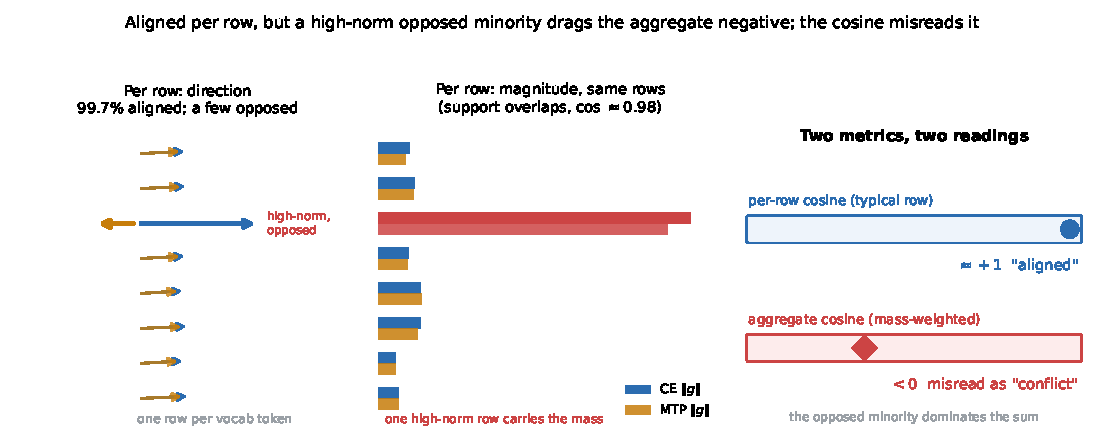
\includegraphics[width=\linewidth]{figures/fig0_schematic.pdf}
\caption{\textbf{Most rows agree; a high-norm minority sets the sign} (schematic; illustrative proportions, not plotted data). \emph{Left:} row by row (one
row per vocabulary token), the CE and MTP gradients point almost the same way for
$99.7\%$ of rows (per-row cosine $\approx +1$); a tiny high-norm minority (red) is
opposed. \emph{Middle:} both losses deposit their gradient \emph{magnitude} on the
\emph{same} rows (norm-profile cosine $\approx 0.98$), and one high-norm row (red)
carries most of the mass. \emph{Right:} the typical per-row cosine reports
alignment, while the magnitude-weighted aggregate, the standard conflict
diagnostic, is dragged negative by the opposed high-norm minority and is
misinterpreted as conflict. The aggregate is not wrong about the update, but it
cannot say \emph{where} the interference lives: it is set by per-row norms, not by
the directions it averages. The $99.7\%$ on the left is the fraction of rows that are
\emph{not} opposed, and the $\approx +1$ is dominated by the ${\approx}92\%$ of
rows that receive no target in the batch and are exact scalar multiples. On the
${\approx}8\%$ that do carry supervision the median cosine is ${\approx}0.53$
with ${\approx}3$--$4\%$ opposed (Section~\ref{sec:aligned}); those are the quantities the
paper's claims rest on.}
\label{fig:schematic}
\end{figure}

% ---------------------------------------------------------------------------


\section{Related Work}
\label{sec:related}

\paragraph{Multi-token prediction.} Predicting several future tokens jointly
dates to blockwise-parallel decoding and ProphetNet \citep{qi2020prophetnet},
and was revived as a pretraining objective by \citet{gloeckle2024mtp}, who attach
$n$ \emph{independent output heads} to a shared trunk and report improved sample
efficiency and up to $3\times$ faster inference via self-speculative decoding. Two
properties of their result are central to ours: the heads are \emph{separate}
(each future offset gets its own unembedding), and the benefit is
\emph{increasingly useful for larger model sizes}. DeepSeek-V3
\citep{deepseekv3} adopts sequential MTP modules at frontier scale; Medusa
\citep{cai2024medusa} and related work add prediction heads primarily for
speculative decoding \citep{samragh2025future}; and MuToR \citep{gerontopoulos2025mutor} interleaves
learnable register tokens so a frozen backbone can predict future offsets without
architectural change. Across this line, the auxiliary signal is given \emph{its
own capacity}: separate heads, modules, or register tokens. The present work
studies the opposite, minimal case, a single tied output embedding shared
across horizons, precisely because it isolates the interference that
separate-capacity designs avoid; a separate-head variant would localize whether
the effect is intrinsic to head-sharing (we identify this as the primary future
experiment).

\paragraph{Small-scale degradation of MTP.} \citet{zuhri2025top} document that
multi-token objectives can \emph{hurt} next-token modeling at smaller scales, and
propose token-order prediction as an alternative. This degradation is the failure
mode we instrument; our contribution is not to add to the catalogue of when MTP
helps or hurts, but to measure \emph{what the gradient geometry actually looks
like} at the shared head when it hurts, and to show that the standard conflict
diagnostic mischaracterizes it.

\paragraph{Gradient conflict and surgery.} A large multi-task literature treats
negative inter-task gradient cosine as the signature of interference and
projects it away: PCGrad \citep{yu2020pcgrad}, Gradient Vaccine
\citep{wang2021gradvaccine}, and gradient-similarity loss weighting
\citep{du2018auxsim}, with later refinements \citep{sun2023drmgf,shi2023recon}.
These methods operate on \emph{global} (flattened) gradient vectors and target
gradient \emph{direction}. A parallel line instead balances gradient
\emph{magnitude}: GradNorm \citep{chen2018gradnorm} dynamically tunes per-task
gradient norms rather than reprojecting directions. This magnitude-versus-direction
distinction is central to our findings, which locate the operative structure in
per-row gradient norms rather than in the direction the aggregate cosine reports.
Independently, \citet{jiang2023forkmerge} argue that optimization-based
gradient-coordination methods can overlook auxiliary-target generalization, so
that gradient-conflict signals do not by themselves determine negative transfer;
our measurement gives a concrete mechanism for how a conflict diagnostic can
mislead at the output head. Concretely, our per-row measurement shows the global
cosine is a lossy summary there: it reads $\approx 0$ while the per-row structure
is near-perfectly aligned. Conflict surgery therefore has little of the targeted
directional conflict to act on (Appendix~\ref{app:surgery}), not because surgery
is poorly implemented, but because the aggregate is set by per-row norm structure,
not by a directional conflict surgery can reproject.

\paragraph{The output head as a bottleneck.} \citet{yang2018softmax} showed the
softmax output layer is a rank bottleneck on the distributions a model can
express. \citet{godey2026lmhead} recently showed, for a \emph{single} loss, that
backpropagating through the low-rank output head destroys most of the gradient's
norm, a norm-space single-loss bottleneck. Our result is the direction-space,
\emph{multi-loss} complement: we ask what a cosine diagnostic reports when two
losses share that head, and find their per-row directions align while their
support appears to compete (an inference, not a direct measurement; see
Section~\ref{sec:discussion}).

\paragraph{Positioning.} Relative to prior work, (i) we provide a per-row
gradient measurement at the tied output projection that a global cosine misses;
(ii) we show the next-token degradation of small-scale shared-head multi-token
training, a documented but unexplained failure mode \citep{zuhri2025top}, co-occurs with \emph{aligned} per-row gradients rather than with directional
conflict, which we read as \emph{support} competition (inferred, not directly
measured); and (iii) our capacity-separated auxiliary
\emph{reduces} the next-token cost in the same spirit as capacity-added fixes,
though in our runs it does not fully recover the CE-only baseline within noise
(neither the standard nor a tuned variant); our contribution is not a fix but the
\emph{diagnostic mechanism}: why conflict-based remedies have nothing to act on
here, and why capacity separation is the lever that helps.

\section{Method}
\label{sec:method}

\subsection{Setup}
We train GPT-2 (124M; 12 layers, $d{=}768$, vocab $50{,}257$ padded to $50{,}304$)
and a 350M variant (24 layers, $d{=}1024$) on FineWeb, tokenized with the GPT-2
BPE. The output projection (\texttt{lm\_head}) is \emph{tied} to the input
embedding by default; Section~\ref{sec:general} reports an untied control. The
primary objective is next-token cross-entropy (CE). The auxiliary multi-token
objective (MTP) supervises the \emph{same tied head} to also predict tokens at
offsets $t{+}2$ and $t{+}3$, with total loss
$\mathrm{CE} + 0.5\,\mathrm{MTP}_2 + 0.25\,\mathrm{MTP}_3$. Evaluation is
\textbf{pure next-token CE on held-out validation} for every variant, so all
reported losses are directly comparable. The loss-comparison runs use a batch of
$16{,}384$ tokens/step for $30{,}517$ steps ($\approx 500$M tokens,
$\approx 4.0$ tokens/parameter at 124M), an intentionally undertrained,
small-batch regime, chosen for controlled comparison and because it is where
shared-head multi-token training is already documented to underperform; we return
to this scope in Section~\ref{sec:discussion}.

\subsection{The per-row instrument}
The output projection has shape $(V, d)$; row $i$ is the weight vector for
vocabulary token $i$. For a validation batch we compute the gradient each loss
deposits on this matrix and, for \textbf{each row}, the cosine between the CE and
MTP row-gradients. We summarize the resulting distribution of $V$ per-row cosines
by its median, the fraction with $\cos < 0$ (directional opposition), and the
fraction with $|\cos| > 0.3$ (appreciable alignment). We contrast these per-row
statistics with the \textbf{aggregate} cosine (the cosine between the two
\emph{flattened} matrix gradients), which is the quantity conventional conflict
diagnostics use. The 47 padding rows ($50{,}304 - 50{,}257$) are masked from all
per-row statistics.

\paragraph{Measurement windows (stated explicitly).} The gradient
instrumentation and the loss comparison come from \emph{different} runs, and we
are careful to keep them distinct. At 124M, the per-row/aggregate trajectory is a
dedicated diagnostic run logged densely over its first $1000$ steps (A1); the
$+0.39$-nat loss gap is the separate $30{,}517$-step training comparison
(Section~\ref{sec:interventions}). Late-training persistence of the alignment is
therefore \emph{not} established at 124M; it is measured directly only at 350M
(single seed), where per-row $|\cos|>0.3$ remains high out to step $87{,}000$
(Section~\ref{sec:rare}). We flag throughout which quantity comes from which run,
and treat single-seed/single-run measurements as such.

\subsection{Direction versus support}
\label{sec:dirsupport}
The distinction the paper turns on: the \textbf{aggregate} cosine measures whether
the summed gradient vectors point the same way; the \textbf{per-row} distribution
measures whether they agree row by row. These can disagree. If two losses each
place their gradient magnitude on a \emph{disjoint} set of rows, then on the rows
where either is active the other is $\approx 0$, the per-row cosines agree where
they overlap, and the flattened aggregate is driven toward orthogonality by the
non-overlap, \emph{without any directional opposition}. We call this
\textbf{support divergence}, and it is invisible to a cosine conflict diagnostic
by construction.

\begin{tcolorbox}[colback=gray!5,colframe=gray!45,boxrule=0.4pt,left=4pt,right=4pt,
  top=3pt,bottom=3pt,fontupper=\small]
\textbf{A two-row illustration.} Take a weight matrix with two rows and let the
CE and MTP gradients be
$g^{\text{ce}}=\big[(1,0),\,(0,0)\big]$ and
$g^{\text{mtp}}=\big[(0,0),\,(1,0)\big]$: each loss loads all its magnitude on a
\emph{different} row. The per-row cosine is undefined on the zero rows and
otherwise never negative, so nothing looks opposed. Yet the flattened vectors
$(1,0,0,0)$ and $(0,0,1,0)$ are orthogonal: the \textbf{aggregate cosine is $0$}.
No row's gradients point in opposing directions; the aggregate reads
``conflict'' purely because the two losses occupy disjoint rows. Support
divergence is this effect at scale.
\end{tcolorbox}

One caveat bounds how far we can push this inference. The aggregate cosine is
\emph{magnitude-weighted} (it is the cosine of the summed, flattened gradients),
whereas the per-row median and the $\cos<0$ fraction are \emph{unweighted} over
rows. A near-zero aggregate with a per-row median of $+1$ is therefore consistent
with (a) disjoint magnitude support across rows, but also with (b) a small number
of high-norm rows being off-axis while the many low-norm rows align, i.e.\ the
$0.33\%$ opposed-by-count figure does not bound the opposed \emph{mass}. Our
committed measurements store per-row cosines but not per-row gradient norms, so we
cannot separate (a) from (b) here; we report support divergence as the reading
most consistent with the full pattern (including the emergent decoupling and the
untied-head control) and flag the direct per-row-norm measurement that would
settle it as future work (Section~\ref{sec:discussion}).

\subsection{Calibration}
To confirm the instrument is not trivially reporting alignment, we run a control
(A3) that measures CE against an unrelated L1 regularizer on the same head. A
well-calibrated instrument should read near-zero alignment for two unrelated
losses.

\section{Experiments and Results}
\label{sec:results}

\subsection{Per-row gradients are predominantly aligned on the rows that carry supervision}
\label{sec:aligned}
\paragraph{The honest denominator: active rows.} Because CE and the shared MTP
loss read the \emph{same} logits from the \emph{same} hidden state, a vocabulary
row that is not a target anywhere in the measurement batch has
$g^{\mathrm{mtp}}_i = 0.75\,g^{\mathrm{ce}}_i$ exactly (the two objectives differ
only in their target-indicator terms, and $0.75 = 0.5{+}0.25$ is the summed
auxiliary weight; the empirically measured norm ratio
$\lVert g^{\mathrm{mtp}}_i\rVert/\lVert g^{\mathrm{ce}}_i\rVert$ on such rows is
$0.750$, which is itself a check that all horizons use the same hidden state). Such rows
are scalar multiples with cosine identically $+1$, and they dominate the count. We
therefore classify rows by \emph{target presence}, not by a cosine threshold: a
row is \emph{active} iff $\lvert\lVert g^{\mathrm{mtp}}_i\rVert/\lVert
g^{\mathrm{ce}}_i\rVert - 0.75\rvert > 0.01$. By this construction
${\approx}88$--$92\%$ of rows are parallel and only \textbf{${\approx}8$--$12\%$
are active} (the exact fraction is batch-relative; see below). Restricted to the
active rows, the median per-row cosine is \textbf{${\approx}0.53$} (Muon
$0.529{\pm}0.006$, AdamW $0.547{\pm}0.013$, $n{=}3$), \textbf{${\approx}3\%$} are
opposed, and ${\approx}83\%$ exceed $\cos>0.3$. Over the full vocabulary the same
run reads a median of $+1.00$, $0.33\%$ opposed, and $98.4\%$ above $|\cos|>0.3$
against a $0.42\%$ calibrated control (Figure~\ref{fig:perrow}); these are the
construction-inflated numbers, reported only to calibrate against the control on a
common denominator. The active-row median of ${\approx}0.53$ is the honest measure
of directional alignment, and it is still well above zero, in sharp contrast to the
near-zero aggregate. Crucially, the active-row correction does \emph{not} affect
the mechanism in Section~\ref{sec:emergent}, which is mass-weighted: the parallel
rows carry only ${\approx}4\%$ of the gradient-magnitude mass, so the norm-profile
cosine ($0.98$) and opposed-norm fraction ($0.60$/$0.69$) are identical whether
computed over all rows or active rows only. The interference lives among the active rows;
restricting to them makes the finding sharper, not weaker.

\begin{figure}[t]
\centering

\includegraphics[width=\linewidth]{figures/fig1_perrow_histogram.pdf}
\caption{\textbf{Per-row CE/MTP gradients on the output projection are aligned on
the rows that carry supervision.} Main panel: distribution of \emph{signed} per-row
cosines over the active rows (median ${\approx}0.53$; ${\approx}3\%$ opposed, in
red). Inset: the full-vocabulary distribution, whose median is $+1.00$ because
${\approx}88$--$92\%$ of rows are parallel by construction ($g^{\mathrm{mtp}} =
0.75\,g^{\mathrm{ce}}$ for any row with no target in the batch, since CE and the
shared MTP loss read the same logits). Right: a CE-vs-L1 control reads $0.42\%$ of
rows above $|\cos|>0.3$ versus $98.4\%$ full-vocab for CE-vs-MTP; on active rows the
comparison is ${\approx}83\%$ versus the control, still a large calibration gap.
GPT-2 124M, step 1000, $50{,}257$ vocab rows (47 padding rows masked). The
mass-weighted mechanism (Section~\ref{sec:emergent}) is unaffected by the
active-row restriction because parallel rows carry only ${\approx}4\%$ of the
gradient mass.}
\label{fig:perrow}
\end{figure}

\subsection{The aggregate cosine decouples from per-row alignment during training}
\label{sec:emergent}
The aggregate cosine nonetheless reads $\approx 0$ ($-0.08$ at step 1000).
Tracking both metrics over training (Figure~\ref{fig:emergent}) shows this is not
a fixed property: at initialization the aggregate and per-row alignment
\textbf{agree at $\approx +0.99$}, and the aggregate then crosses zero early (between steps $100$ and $150$ under Muon, and between $150$ and $200$ under AdamW) while the per-row median holds at $\approx +1$ for the remainder of the
$1000$-step diagnostic window (late-training persistence is shown separately at
350M, Section~\ref{sec:rare}). These trajectories are a single diagnostic run per
optimizer; the close agreement between two different optimizers is the
replication we have.

We can pin down \emph{how} the aggregate collapses without any additional runs,
using an exact identity. The aggregate cosine is a magnitude-weighted average of
the per-row cosines, $\text{agg}=\sum_i w_i\cos_i$ with weights
$w_i=\lVert g^{\text{ce}}_i\rVert\lVert g^{\text{mtp}}_i\rVert/(\lVert
G^{\text{ce}}\rVert\lVert G^{\text{mtp}}\rVert)\ge 0$. If gradient magnitude were
spread evenly across rows, the weights would be equal and the aggregate would
equal the \emph{plain mean} of the per-row cosines. That mean is $+0.94$ (Muon)
and $+0.96$ (AdamW), whereas the actual aggregate is $-0.08$ and $-0.28$
(Figure~\ref{fig:normdecomp}). The entire $\approx\!1.0$ gap between ``aggregate
if norms were flat'' and the real aggregate is therefore attributable to the
per-row \emph{norm} structure, not to the typical per-row direction: the standard
diagnostic is reporting a magnitude-weighting artifact, which is the paper's
central point made quantitative.

The weights are unnormalized, and their sum is itself informative. Writing
$a_i=\lVert g^{\text{ce}}_i\rVert$ and $b_i=\lVert g^{\text{mtp}}_i\rVert$, we
have $\sum_i w_i=\langle a,b\rangle/(\lVert a\rVert\lVert b\rVert)=\cos(a,b)$,
which is exactly the \emph{norm-profile cosine} $\rho_{\text{norm}}$ defined
below. The aggregate therefore factors exactly as
\begin{equation}
\text{agg}=\sum_i w_i\cos_i
      =\underbrace{\Big(\textstyle\sum_i w_i\Big)}_{\rho_{\text{norm}}}
       \cdot\underbrace{\frac{\sum_i w_i\cos_i}{\sum_i w_i}}_{\langle\cos\rangle_{\text{mass}}}
      =\rho_{\text{norm}}\,\langle\cos\rangle_{\text{mass}},
\end{equation}
the product of how much the two losses' norm profiles overlap and the
mass-weighted mean of the per-row cosines. Numerically this is
$-0.08 = 0.98\times(-0.082)$ (Muon) and $-0.28 = 0.98\times(-0.286)$ (AdamW). The
two ``disambiguating statistics'' we introduce next are therefore not competing
hypotheses but the two exact factors of the aggregate: support overlap is the
total weight $\rho_{\text{norm}}$, and opposition is carried by
$\langle\cos\rangle_{\text{mass}}$.

What the identity does \emph{not} settle is which norm structure is responsible.
A negative aggregate requires the opposed minority ($\cos<0$, $\approx 0.33\%$ of
rows) to carry \emph{some} weight, so two mechanisms are a priori compatible with
the aligned-median-plus-negative-aggregate pattern: (a) \emph{support
divergence}, where CE and MTP load their magnitude onto increasingly disjoint
rows, making the products $w_i$ small precisely where each gradient is large; and
(b) a small number of \emph{high-norm opposed rows} dominating the weighted sum.
Separating (a) from (b) needs the per-row gradient \emph{norms}, which the earlier
runs do not store, so we measure them directly with a drop-in instrument
(\texttt{measure\_norm\_support.py}) that logs per-row norms and reports two
disambiguating statistics on the same short diagnostic pass: the
\emph{norm-profile cosine} (the cosine of the two per-row norm vectors; $\approx0$
under support divergence, $\approx1$ if the losses load the same rows) and the
\emph{opposed-norm fraction} (the share of $\lVert g^{\text{ce}}_i\rVert\lVert
g^{\text{mtp}}_i\rVert$ mass on rows with $\cos<0$). Across three seeds per
optimizer, the norm-profile cosine is $0.98$ (Muon $0.979\pm0.003$, AdamW
$0.977\pm0.007$): CE and MTP load the \emph{same} rows, so support does
\emph{not} diverge. Yet the opposed-norm fraction is $0.60\pm0.03$ (Muon) and
$0.69\pm0.01$ (AdamW): the majority of the magnitude mass sits on the opposed
minority. Mechanism (b) holds, and it holds under both optimizers, with AdamW
cancelling more strongly than Muon (Figure~\ref{fig:normsupport}); the difference
in opposed-norm fraction ($0.69$ vs $0.60$) is significant across seeds (Welch
$t{=}5.4$, $p\approx0.015$), so the magnitude is genuinely optimizer-dependent
while the mechanism is shared. The near-zero
aggregate is a norm-weighted cancellation by a high-norm opposed minority, not
disjoint support.

\begin{figure}[t]
\centering

\includegraphics[width=0.86\linewidth]{figures/fig7_norm_support.pdf}
\caption{\textbf{The aggregate is set by a high-norm opposed minority, not by
disjoint support} ($n{=}3$ seeds per optimizer, step $1000$, $50{,}257$ real
vocabulary rows). \emph{Left:} the norm-profile cosine (the cosine of the two
per-row gradient-norm vectors) is $\approx 0.98$ for both optimizers, so CE and
MTP load the same rows; support does not diverge. The actual aggregate cosine
nonetheless sits negative, and the arrow marks the collapse. \emph{Right:} the
opposed-norm fraction, the share of $\lVert g^{\text{ce}}_i\rVert\lVert
g^{\text{mtp}}_i\rVert$ mass on rows with $\cos<0$, is above one half for both
optimizers ($0.60$ Muon, $0.69$ AdamW): the opposed minority carries most of the
magnitude mass. AdamW cancels more strongly than Muon; the mechanism is identical,
the magnitude optimizer-dependent.}
\label{fig:normsupport}
\end{figure}

\paragraph{Which rows carry the cancellation.} The opposed mass is not spread
thinly: on the Muon seed-42 pass, $140$ opposed rows ($0.28\%$ of the vocabulary)
carry $60.7\%$ of the total $\lVert g^{\text{ce}}_i\rVert\lVert g^{\text{mtp}}_i\rVert$
mass, and just $47$ rows account for two-thirds of \emph{all} gradient mass
(Figure~\ref{fig:tokenlorenz}, left). Decoding those rows shows they are the most
frequent function words and punctuation: the four highest-mass opposed rows are
\texttt{.}, the newline, \texttt{\ the}, and \texttt{,}, which alone carry
${\approx}41\%$ of the mass, followed by \texttt{\ of}, \texttt{\ to}, \texttt{\ and},
and \texttt{\ a} (Figure~\ref{fig:tokenlorenz}, right). This is the expected locus:
these tokens are ubiquitous next-token \emph{and} future targets, and their
next-token and future-token continuation distributions genuinely differ, so the
CE and MTP gradients on their output rows point in different directions while both
being large. The cancellation is concentrated on a handful of high-frequency rows,
not diffuse across the tail.

\begin{figure}[t]
\centering

\includegraphics[width=\linewidth]{figures/fig_token_lorenz.pdf}
\caption{\textbf{The cancellation is carried by a few high-frequency rows.}
\emph{Left:} Lorenz curve of the per-row gradient mass
($\lVert g^{\text{ce}}_i\rVert\lVert g^{\text{mtp}}_i\rVert$, ranked descending);
$47$ rows account for two-thirds of all mass (dashed line), against the
line of equality (dotted). \emph{Right:} the highest-mass opposed rows, decoded,
are the most frequent function words and punctuation; the top four carry
${\approx}41\%$ of the total mass. Muon, seed 42, step 1000.}
\label{fig:tokenlorenz}
\end{figure}

\begin{figure}[t]
\centering

\includegraphics[width=0.72\linewidth]{figures/fig2_emergent_divergence.pdf}
\caption{\textbf{The aggregate and per-row alignment start together and
decouple.} Both metrics begin at $\approx +0.99$; within ${\sim}200$ steps the
aggregate (matrix-level) cosine falls below zero (crossing between steps
$100$--$150$ for Muon and $150$--$200$ for AdamW) while per-row alignment stays
high. The per-row curve is the full-vocabulary $|\cos|>0.3$ fraction
($\approx 0.98$); on active rows the level is lower ($\approx 0.83$, Section~\ref{sec:aligned})
but the decoupling from the aggregate is identical: the aggregate goes
negative under either denominator. One diagnostic run per optimizer (Muon solid,
AdamW dashed); the agreement between two optimizers is the replication.}
\label{fig:emergent}
\end{figure}

\begin{figure}[t]
\centering

\includegraphics[width=0.62\linewidth]{figures/fig6_norm_decomposition.pdf}
\caption{\textbf{Per-row norm structure, not the typical cosine, sets the
aggregate.} For each optimizer: the median per-row cosine ($+1.00$), the plain
\emph{mean} per-row cosine (which equals the aggregate the standard diagnostic
would report if gradient magnitude were spread evenly across rows), and the
\emph{actual} aggregate cosine. The mean is strongly positive ($+0.94$/$+0.96$)
while the actual aggregate is negative ($-0.08$/$-0.28$); the gap is due entirely
to per-row norm weighting. Single diagnostic run per optimizer, step $1000$,
$50{,}257$ real vocabulary rows.}
\label{fig:normdecomp}
\end{figure}

\subsection{The pattern is general, and survives untying}
\label{sec:general}
High per-row alignment is \textbf{not unique to the output head}. Across all 74
weight matrices (Figure~\ref{fig:perlayer}), attention and MLP matrices also show
high per-row alignment (many above 0.8), frequently with strongly \emph{negative}
aggregate cosine (down to $-0.78$). The output head is distinctive only in being
the point of \textbf{maximum} per-row alignment ($0.984$) sitting nearest
aggregate-zero, and, more importantly, in being the matrix that \emph{directly
produces the logits}. The head matters not because the metric singles it out, but
because interference there is paid directly in next-token loss. Alignment also
\textbf{persists when the head is untied} (A4: $99.3\%$ of rows above threshold,
versus $98.7\%$ tied at the matched step), so it is a property of the
output-projection gradient ($h^\top \partial\mathcal{L}/\partial\text{logits}$),
not an artifact of weight tying. These two percentages are \emph{full-vocabulary}
and therefore construction-floored (${\geq}75\%$ of rows are parallel by
construction); the untied run did not commit per-row norms, so we cannot restate
them on the active-row denominator, and we report them only as a point check that
untying does not \emph{reduce} alignment. The evidentiary weight of this check is
modest in any case: the soft-label identity (Section~\ref{sec:interventions}) predicts
untied-persistence \emph{a priori}, since that identity never references tying.
The per-layer generality (Figure~\ref{fig:perlayer})
and the untied-head comparison are each \emph{single-run} measurements at a fixed
step; we report them as point observations, not seed-replicated estimates (only
the 124M CE-vs-MTP loss gap is replicated across seeds).

We are deliberate about what this generality does and does not license. The
same qualitative signature (high per-row alignment with a non-positive aggregate) appears across the network, and at many matrices the aggregate is
\emph{strongly} negative (to $-0.78$), not merely near zero. This means the
per-row/aggregate gap is a fairly generic property of these structured gradient
matrices, so a near-zero aggregate on its own is \emph{not} a specific signature
of two-loss interference. What is specific to the output head is that it is the
one matrix whose per-row gradients are the CE and MTP gradients directly, whose
norm-weighted opposition we measure end to end (Figure~\ref{fig:normsupport}),
and whose interference is paid immediately in next-token loss. We do not
adjudicate the per-row norm structure of the strongly-negative aggregates
elsewhere in the network; a per-row account of those is beyond what our
measurements settle.

\begin{figure}[t]
\centering

\includegraphics[width=0.66\linewidth]{figures/fig3_perlayer.pdf}
\caption{\textbf{High per-row alignment is general across the network.} Per-row
alignment vs aggregate cosine for all 74 weight matrices. The output head (star)
is the maximum and sits nearest aggregate-zero, but attention/MLP matrices show
the same pattern, many with strongly negative aggregate cosine.}
\label{fig:perlayer}
\end{figure}

\subsection{Adding shared MTP degrades next-token loss; no auxiliary recovers it}
\label{sec:interventions}
Adding the shared MTP objective degrades next-token validation loss from
$\mathbf{3.985 \pm 0.014}$ (CE-only, $n{=}5$) to $\mathbf{4.377 \pm 0.021}$
($n{=}3$): a \textbf{$+0.39$ nat} (${\approx}10\%$) increase. On the three seeds
the two conditions share ($42,123,456$), a paired test gives a mean gap of
$\mathbf{0.382}$ nats (per-seed $0.397/0.380/0.370$), $t{=}50.0$,
$\mathbf{p \approx 4.0\times10^{-4}}$ ($\text{df}{=}2$); treating the conditions
as independent (Welch, CE-only minus shared-MTP, using all $n{=}5$ and $n{=}3$
seeds) gives $t = -28.8$ (negative because CE-only is the lower loss),
$p \approx 8\times10^{-5}$ with a $95\%$ CI on the difference of
$[0.35, 0.43]$ nats. The gap is large relative to the seed-to-seed spread
(within-condition sd $\approx 0.01$--$0.02$), which is what makes it detectable
at these small $n$; we report the effect as the $0.39$-nat loss increase itself
rather than a standardized effect size, since the latter is inflated by the tight
reproducibility of a controlled testbed. With $n{=}3$ per condition and this
spread, the minimum difference we have ${\approx}80\%$ power to detect is
$\Delta\approx0.05$ nats; the headline gap is ${\sim}8\times$ that floor, so it is
detected with room to spare, whereas differences below ${\approx}0.05$ nats
(relevant to the tuned auxiliary below) are at or under our detection limit. We
report uncorrected $p$-values for the $k{=}5$ variant-vs-baseline comparisons;
under a Holm correction at $\alpha{=}0.05$ the shared-MTP, stop-gradient,
standard-contrastive, and NextLat results remain significant, while only the
tuned-auxiliary comparison ($p\approx0.19$) does not survive, consistent with its
effect sitting below the detection floor. Detaching
the auxiliary from the head via stop-gradient makes it \emph{worse} ($4.493$,
$\Delta{+}0.508$, $p < 10^{-4}$), not better, which points to a norm-weighting/capacity account rather than directional conflict (we note this is a data
point, not a proof: stop-gradient also removes the auxiliary's ability to shape
the shared representation, which is a competing reason it could hurt). The
$n{=}5$ CE-only and $n{=}3$ shared-MTP conditions share three seeds ($42,123,456$);
the two extra CE-only seeds ($789,1337$) were run for a tighter baseline and no
MTP seeds were dropped. Capacity-separated auxiliaries reduce but do \textbf{not}
recover the baseline. The \emph{standard} layer-split contrastive auxiliary
($\mathrm{G}_{\text{nce}}$: an InfoNCE-style contrastive loss applied to an
intermediate layer, giving the auxiliary its own representation capacity instead
of sharing the output head) reaches $4.024$ ($\Delta{+}0.039$, $p \approx 0.010$),
statistically distinguishable from A, i.e.\ a genuine non-recovery. A
hyperparameter-tuned variant reaches $4.003$ ($\Delta{+}0.018$) but is \emph{not}
statistically separable from A at $n{=}3$ ($p \approx 0.19$): for this variant we
can claim neither recovery nor non-recovery, and we rest the capacity conclusion
on the standard variant. A latent-prediction baseline (NextLat: the auxiliary
predicts the \emph{hidden state} at future offsets rather than their tokens, so it
never touches the output head) lands at $4.037$ ($\Delta{+}0.051$, Welch
$p{\approx}0.018$) (Figure~\ref{fig:interventions}).

\begin{figure}[t]
\centering

\includegraphics[width=0.66\linewidth]{figures/fig4_interventions.pdf}
\caption{\textbf{No auxiliary recovers the baseline; MTP degrades it most.} Final
next-token validation loss by variant (points = seeds). Shared MTP degrades CE by
$\Delta{+}0.39$; stop-grad by $\Delta{+}0.51$; no capacity-separated auxiliary
recovers the CE-only baseline within noise.}
\label{fig:interventions}
\end{figure}

Conflict-targeted gradient surgery also does not recover the baseline, and this
is a stronger statement than ``there was nothing to remove.'' The opposed rows
are negligible by count ($0.3\%$) but carry the majority of the gradient mass
($60$--$69\%$), and a projection acts on the mass-weighted vector, so surgery had
a great deal to project away; per-row Gram--Schmidt on the head targets exactly
those opposed rows and still recovers nothing. The measured opposition is
mass-dominant and causally inert. Because those runs are single-seed with a
numerical-drift caveat, we report them in full in Appendix~\ref{app:surgery}
rather than resting any claim on them.

\subsection{The apparent rare-token alignment is a construction artifact; the pattern holds at 350M}
\label{sec:rare}
Measured over the full vocabulary, per-row alignment appears \emph{higher} for
rarer tokens: the rarest quintile averages $0.98$ mean $|\cos|$ versus $0.86$
for the most-common quintile (Figure~\ref{fig:tokenfreq}, left). This effect is
an \emph{artifact of the construction floor}. Rare tokens are almost never
targets in a measurement batch, so they are overwhelmingly parallel-by-construction
($\cos=+1$): the active fraction falls from ${\approx}25\%$ in the common quintile
to ${\approx}1.5\%$ in the rarest. Restricted to active rows, the apparent
gradient disappears: active-row mean $|\cos|$ is essentially flat across
frequency quintiles ($0.51$--$0.54$ for Muon, $0.52$--$0.60$ for AdamW;
Figure~\ref{fig:tokenfreq}, right), with only a weak residual (Spearman
$\rho{\approx}0.12$ between token id and active-row $|\cos|$). We therefore
\emph{retract} the rare-token-alignment reading: the full-vocabulary ordering
reflects how many rows are parallel by construction, not a frequency-dependent
alignment. The
aligned-per-row-with-negative-aggregate picture holds qualitatively at
\textbf{350M} (single seed): CE-only $3.752$, shared-MTP $4.129$ ($\Delta{+}0.378$).

The 350M runs are the paper's only \emph{late-training} per-row measurement,
logged out to step $87{,}000$. The instrument computes the same quantity in both
runs (the per-row cosine between the CE gradient and the MTP gradient on the output projection) regardless of which objective the model was trained with
(the MTP gradient is computed at measurement time for both). Measured this way,
the shared-MTP-trained model holds $|\cos|>0.3$ at $98.9\%$ of rows at step
$87{,}000$, and the CE-only-trained model reads $94.5\%$ at the same step. These
are \emph{full-vocabulary} figures and thus construction-floored: with ${\geq}75\%$
of rows parallel by construction, the informative range is the remaining
${\approx}25$ percentage points, within which the MTP-trained model sits near the
top and the CE-only model ${\approx}4$ points lower (coarse, but not vacuous),
stated here at its true resolution (the 350M runs committed only summary statistics,
so an active-row restatement is not recoverable from the saved data). That
the CE-only model \emph{also} shows high CE/MTP alignment this late indicates the
alignment is an intrinsic property of the output-projection gradient geometry,
not something the MTP objective induces. Both are single seeds, so we treat the
per-row persistence as illustrative (consistent with alignment not decaying over a
long horizon), not established. The 350M \emph{loss} gap ($\Delta{+}0.378$ above)
is a next-token-loss number, unaffected by the active-row denominator, and it is
this scale-stability of the gap (${+}0.392$ at 124M, ${+}0.378$ at 350M) that
Section~\ref{sec:interventions} builds on.

\begin{figure}[t]
\centering

\includegraphics[width=0.6\linewidth]{figures/fig5_token_frequency.pdf}
\caption{\textbf{The rare-token alignment effect is a construction artifact.}
Left: over the full vocabulary, mean per-row $|\cos|$ rises from common to rare
tokens (both optimizers); this is the apparent effect. Right: restricted to active
rows (those carrying a target), the effect vanishes and mean $|\cos|$ is flat
across frequency quintiles; the grey bars show the active fraction collapsing
from ${\approx}25\%$ (common) to ${\approx}1.5\%$ (rare), which is what drives the
full-vocabulary trend. Single run per optimizer, step 1000, GPT-2 124M.}
\label{fig:tokenfreq}
\end{figure}

\section{Discussion}
\label{sec:discussion}

\paragraph{What the measurements establish.} In this regime (a single shared tied output projection, ${\leq}350$M, undertrained) the standard cosine
conflict diagnostic misreads the CE/MTP interaction. On the rows that carry a
target the per-row gradients are aligned (active-row median cosine ${\approx}0.53$,
${\approx}3$--$4\%$ opposed; the full-vocabulary median is $+1$ only because
${\approx}92\%$ of rows are scalar multiples by construction), the aggregate
is $\approx 0$ or negative, and the two decouple during training. Instrumenting the per-row norms shows the aggregate is set by a high-norm opposed minority ($\approx0.3\%$ of all rows, carrying $60$--$69\%$ of the mass), not by disjoint support. The losses load the same rows (norm-profile cosine $0.98$) but oppose on the few rows that dominate the weighted sum. Crucially, the next-token degradation is large and
unambiguous, yet neutralizing that directional opposition does not remove it. The surgery
baselines in Appendix~\ref{app:surgery} recover nothing, which is consistent
with the opposed minority not being the fixable lever. Under the soft-label reading
this is expected for a sharper reason than opposition that carries the mass yet is
causally inert: the objective's \emph{minimizer has moved} to the mixture $q^{*}$,
and reprojecting gradients does not move it back. For symmetric PCGrad the argument
is exact: at a stationary point of the summed loss $g_{\text{CE}} = -g_{\text{MTP}}$,
both project to zero, and the mixture optimum stays stationary. Our asymmetric
head-only Gram--Schmidt is not a fixed point of those dynamics in the same way, so
there the empirical null is the evidence, and the natural reading is that a head-only
correction cannot undo a shifted optimum while the trunk keeps receiving the full
mixture gradient and shaping representations toward $q^{*}$. Capacity separation helps precisely because the auxiliary no longer forces one set of logits to serve every horizon,
though in our runs it reduces rather than eliminates the gap.

\paragraph{The stop-gradient result cuts the other way.}
One intervention appears to contradict the shifted-optimum account, and we state it
plainly rather than leave it to a reader. If the head's blended target were the
whole story, then $\mathrm{sg}(W)h$ should help: the head is freed to minimize pure
next-token cross-entropy given the representation it is handed. Instead
stop-gradient is the worst of the auxiliary conditions in
Table~\ref{tab:conditions} ($4.493$, $\Delta{+}0.508$ against shared MTP's
$\Delta{+}0.392$); only the gradient-surgery and optimizer-coverage variants of
Appendix~\ref{app:surgery} sit higher. The reason we cannot read this as a refutation is
that the probe moves two quantities at once. It removes the head's mixture target,
which the account predicts should help, and it also stops the head from co-adapting
to a trunk that is still being shaped by the full mixture gradient, which should
hurt. The observed sign says the second effect is the larger one; it does not say
the first is absent. Separating them needs an intervention that removes the mixture
target from the head \emph{without} decoupling head and trunk, which is what the
separate-head variant in \emph{Future work} does. Until then we treat the
stop-gradient number as evidence against the naive head-detach fix and as
uninformative about the mixture account itself.

Beyond the diagnostic result, an exact rewrite shows the shared-head objective is
soft-label cross-entropy toward a next-and-future-token mixture
(Section~\ref{sec:softlabel}), and a zero-parameter estimate of the implied KL cost,
computed entirely from the CE-only model's own distributions, matches the observed
degradation within run noise at the lower auxiliary weights while the full-mixture
variant reproduces ${\approx}88$--$89\%$ of the matched within-sweep gap at full weight, leaving a
${\approx}0.04$-nat residual attributable to the estimator's remaining downward
proxy bias and/or a small genuine non-mixture component
(Section~\ref{sec:mixturetest}). The anchored weight sweep shows the degradation
scales with the auxiliary weight as this account predicts, as a weight-proportional
interference account would also predict; the two shapes are indistinguishable at our
noise level.

\paragraph{Two failure modes, one instrument.} The aggregate cosine misleads in
two opposite directions depending on the optimizer, and the paper's central claim
is that both are failures of the \emph{same} diagnostic. Under Muon the aggregate
is ${-}0.08$ to ${-}0.19$ across measurement batches, close enough to zero at its shallowest reading (${-}0.08$) that a conflict diagnostic reads
``no interference,'' a \emph{false negative}: the next-token loss degrades by
$0.39$ nats regardless. Under AdamW the aggregate is ${-}0.28$ (${-}0.30$ to
${-}0.34$ over the norm-committing seeds), negative enough to trip a conflict flag,
and the surgery runs are \emph{consistent with} a false positive: projecting out
exactly this opposition recovers nothing (Appendix~\ref{app:surgery}). Those runs are
single-seed, with a drift envelope ($0.02$--$0.04$ nats) that overlaps the effects
they would need to resolve, so this arm is suggestive rather than established; the
matched-seed replication that would settle it is future item~3 below. A practitioner reading only the head's aggregate would conclude
``safe to add MTP'' under Muon and ``apply surgery'' under AdamW, and both
conclusions are wrong, the first demonstrably and the second on suggestive
evidence. The false negative is specific to the head: as
Section~\ref{sec:general} notes, an all-parameter aggregate would very
likely read clearly negative under both optimizers, so the misread is of
\emph{where} interference lives rather than of whether any is present. The instrument
does not merely lose power; it points the wrong way, and
which way depends on an optimizer choice unrelated to whether interference is
present. This is why the per-row and per-norm decomposition, not a scalar
threshold on the aggregate, is what the regime requires.

\section{Limitations}
\label{sec:limitations}
We state the boundaries of the result under four headings: what the scope of the
claim is, what is not established about mechanism, what biases the estimator
carries, and where the statistics are thin.

\paragraph{Scope.} Every measurement is on a single shared tied output projection
at ${\leq}350$M parameters, in an undertrained, small-batch regime where MTP is
already documented to underperform \citep{gloeckle2024mtp,zuhri2025top}. We do not show that MTP
\emph{as practiced} (with separate per-horizon heads) degrades next-token
modeling. The reason separate heads should help is not that they stop the losses
from sharing rows: the standard designs share one unembedding matrix, so per-row
gradient mixing persists there. It is that per-horizon logits remove the
constraint that one distribution serve every horizon, which is precisely the
optimum shift of Equation~\ref{eq:softlabel}. That makes the separate-head
experiment a clean test of our own account rather than a mere scaling check, since
it holds shared rows fixed and varies only the shared-label ingredient. The
outcome measure is also narrow: we record next-token validation loss, not downstream
task performance, so ``degrades'' should be read as that quantity and no more.

\paragraph{Mechanism.} We do not establish causation between the norm-weighted opposition and the loss increase. We show they co-occur, and that interventions behave as a shifted-optimum account predicts: surgery that removes the opposition does not remove the degradation, and separating capacity helps.
A related gap is one of timing rather than of inference. The per-row and per-norm
measurements are taken early in training, at step $1{,}000$, while the loss
comparisons are at $30{,}517$ steps; late-training persistence of the alignment is
measured directly only at 350M, on a single seed. The aligned-gradient state and
the degraded-loss state are therefore never exhibited in the same measurement at
124M, and the connection between them rests on that persistence rather than on a
co-located observation.

\paragraph{Estimator.} The zero-parameter prediction sits below the observed gap
by $0.035$--$0.046$ nats: within its stated biases, but also within what a small
genuine interference residual would produce. We treat the mixture account as the
leading candidate, not as confirmed, and we name the residual rather than assign
it. The estimate is also truncated rather than fully marginalized, and truncation
biases it upward relative to full marginalization, so a fuller estimate would
lower the prediction and \emph{widen} the residual rather than close it.

\paragraph{Which gradient we measure.} The head is weight-tied, so the gradient our
instrument reads sums the output-projection path and the embedding path
(Section~\ref{sec:instrument}). The embedding path deposits only on rows that already
carry a target, so it lands exactly on the active rows every statistic here is
computed over, and we do not bound its share. Two measurements would close this, and neither needs new
training. One is to recompute the projection path alone, taking the gradient with
respect to the logits and forming $\sum_t \delta_i(t) h_t$ directly. The other is to
commit per-row norms from an untied run, where the head tensor receives the
projection path only. The existing untied run cannot serve, because it committed
full-vocabulary fractions rather than per-row arrays.

\paragraph{Statistics and instrument caveats.} Seed counts are small and uneven: $n{=}5$ for CE-only and the standard $G_{\text{nce}}$ auxiliary, $n{=}3$ for the other four conditions (Table~\ref{tab:conditions}). The auxiliary-weight sweep of Section~\ref{sec:mixturetest} is a single seed throughout, so the strongest quantitative claim in the paper carries no across-seed spread of its own. The untied-head check is one run at $500$ steps
against $30{,}517$ elsewhere. Finally, the full-vocabulary form of the CE-vs-L1
control is threshold-sensitive and we do not rest calibration on it. On the
committed diagnostic run the fraction of rows with $|\cos|$ above $0.1$, $0.2$,
$0.3$ and $0.5$ is $74.9\%$, $35.2\%$, $0.42\%$ and $0$: nearly $35\%$ of
rows fall between the $0.2$ and $0.3$ bins, so the above-$0.3$ figure is
sensitive to exactly where the cut is placed, and it reads $36.2\%$ on the sweep
snapshot. That snapshot committed only these binned fractions, not the underlying per-row cosines. We therefore cannot say whether the two runs differ by a small shift near this quantile or more substantially, and we do not claim the discrepancy is explained. The shape of that distribution is itself unexplained, and we flag it rather than
account for it. Two comparisons bound the problem. Against isotropic vectors in
$d{=}768$ the cosine standard deviation is $0.036$, so almost no rows should clear
$0.1$, yet $74.9\%$ do: the rows are far more aligned than chance. But the profile is
also \emph{sharper} than any low-dimensional-span model predicts. Suppose both gradients were random within a shared
$k$-dimensional subspace. Any $k$ that reproduces the
above-$0.1$ fraction (within $5$ points of the observed $74.9\%$) forces the ratio of
the above-$0.2$ to the above-$0.3$ fraction to at most ${\approx}2$. The observed
ratio is $84$. Larger $k$ can produce a sharp ratio, but only by putting far too
little mass above $0.1$. The
best-fitting single $k$ is $23$, and it still overpredicts the above-$0.3$ fraction by
a factor of ${\approx}37$. So neither a chance model nor a shared-span model
reproduces the cliff, and we do not have per-row cosines from this run to diagnose it.
The control's role is to show that an \emph{unrelated} loss pair yields a near-zero
aggregate ($0.002$), not to quantify a per-row distribution. The unexplained shape
therefore does not bear on the calibration claim. It remains a loose end: committing
per-row cosines for the control is the measurement that would close it. What both runs agree on is the property the control
exists to establish: the aggregate cosine is near zero either way ($+0.002$ and
$-0.011$). This is why the active-row control of Section~\ref{sec:calib} is the
one we report.

\paragraph{Future work.} Five directions would broaden the scope from ``the diagnostic misreads this
regime'' toward a causal, general statement.
\begin{enumerate}
\item[(1)] A \textbf{separate-head MTP} variant, to localize whether the
      degradation is intrinsic to head-sharing.
\item[(2)] A \textbf{co-located measurement} at $30{,}517$ steps plus a 124M
      CE-only per-row baseline, to replace the timing assumption
      noted under \emph{Mechanism} above with a direct observation, and $n{=}3$ at
      350M to turn the single-seed scale observation into a measured trend.
\item[(3)] \textbf{Matched-seed, single-pass gradient surgery} at $n{=}3$, to
      remove the numerical-drift caveat.
\item[(4)] A \textbf{tighter KL estimate} (full marginalization or larger $k$,
      and better-trained proxy models), to bound the $0.035$--$0.046$-nat
      residual from the prediction side rather than the measurement side. The
      highest-value single piece is \textbf{estimating $P_3$ directly} instead of
      substituting $P_2$. That is the one bracket arm whose direction we have not
      bounded. Our own offset-3 cross-entropies suggest the substitution biases the
      prediction downward, so removing it could shrink the residual rather than
      merely bound it.
\item[(5)] \textbf{Committing per-row cosines for the control} at both
      checkpoints, which is what would settle the threshold-sensitivity
      question raised under \emph{Statistics and instrument caveats} above. Both snapshots are preserved,
      but neither stores the per-row array.
\end{enumerate}

\section{Conclusion}
\label{sec:conclusion}
Cosine similarity between task gradients is the default instrument for detecting
interference in multi-task and auxiliary-loss training. We showed that at a language model's shared, tied output projection this instrument is misleading, in three respects. The per-row CE and MTP gradients are aligned in direction on the rows that carry a target (active-row median cosine ${\approx}0.53$; the full-vocabulary median is $+1$ because most rows are scalar multiples by construction). The aggregate cosine is driven negative by a high-norm opposed minority ($\approx0.3\%$ of rows carrying most of the mass), not by a broad directional conflict. And the two metrics decouple during training.
Adding the shared auxiliary degrades next-token loss substantially, and the
surgery baselines we ran, single-seed and reported in
Appendix~\ref{app:surgery}, do not repair it. The aggregate is
set by per-row gradient norms, not by the per-row directions the cosine averages,
a distinction that explains why conflict-targeted surgery does not help here and
why capacity separation does. An exact rewrite of the objective supplies the
complementary positive account: the shared head optimizes cross-entropy against a
next-and-future-token mixture, so its optimum has moved, and a zero-parameter estimate of the
resulting KL cost reproduces most of the measured degradation, undershooting it by
$0.035$--$0.046$ nats at full auxiliary weight. On this reading the degradation is a predictable consequence of the objective rather than a pathology of optimization. Gradient surgery is then inert: exactly so for symmetric projection, and empirically so for the head-only variants we test, where the trunk continues to receive the full mixture gradient. We deliver the result
on a fully reproducible testbed with a committed statistics script, and we are
explicit about the shared-head, small-scale scope and the experiments that would
extend it.


\section*{Reproducibility Statement}
All results are computed from committed result JSONs by \texttt{analysis/stats.py}; all
data figures are regenerated from the same JSONs by \texttt{figures/make\_figures.py}
(the conceptual schematic, Figure~\ref{fig:schematic}, by \texttt{figures/make\_schematic.py}).
Code, data-loading, pinned dependencies (\texttt{requirements.txt}), and a
\texttt{README} with exact run commands are available at
\repourl{}. The optimizer (Muon) is pinned to
commit \texttt{056a3c5869cf}. Every training and measurement run reported here was
performed on a single rented NVIDIA H100, booked through the Prime Intellect compute
exchange on hardware operated by Verda (DataCrunch). Across the $74$ committed runs the recorded
wall-clock totals $196{,}501$ seconds, or ${\approx}54.6$ H100-hours; that
counts the runs whose JSONs ship here and excludes exploratory and failed
attempts, which were not committed and whose time we did not log. (That $74$ is
coincidental and unrelated to the $74$ weight matrices of
Section~\ref{sec:general}.) This work received no external funding. Scope and caveats are stated in
Section~\ref{sec:intro} and Section~\ref{sec:limitations}.

\paragraph{Use of large language models.} A large language model was used as a
writing and analysis assistant: drafting and revising prose, generating
figure-plotting and statistics code, and cross-checking arithmetic against the
committed result files. It was not used to generate data, and no experimental
result, number, or citation in this paper originates from a model without being
recomputed from the committed JSONs or verified against the cited source. The
author is responsible for all claims.



\bibliography{../../references}
\bibliographystyle{tmlr}

\appendix
\section{Surgery and control baselines (single-seed; reported for completeness)}
\label{app:surgery}

We ran conflict-targeted gradient-surgery methods on the shared-MTP variant to
test directly whether removing directional conflict recovers the baseline.
\textbf{We do not rest the paper's diagnostic result on these runs}; we read
them as consistent-with rather than as evidence, for three
reasons stated up front.
\begin{enumerate}
\item[(i)] Each is a \textbf{single seed} (seed 42).
\item[(ii)] The PCGrad baseline operates on \textbf{all parameters}, whereas
      per-row Gram--Schmidt and Scatter operate on the \textbf{output head
      only}, so they are not strictly comparable.
\item[(iii)] Surgery uses \textbf{two backward passes} under bf16, versus the
      fused single pass of the main runs, introducing a ${\sim}0.02$--$0.04$ nat
      numerical drift comparable to the smaller surgery effects.
\end{enumerate}
With those caveats, the pattern is uniform: no surgery method recovers the
CE-only baseline ($\text{A} = 3.985$), and none improves on the matched
shared-MTP seed ($\text{B@42} = 4.399$). Two of them make it measurably worse.
Per-row Gram--Schmidt at $+0.018$ sits inside the $0.02$--$0.04$ nat drift
envelope, so we read it as no recovery. Scatter at $+0.058$ and PCGrad at
$+0.145$ are outside that envelope, and PCGrad and Pure-Muon also act on all
parameters rather than the head alone. We report the worsening as measured and
do not explain it: removing the opposed component discards gradient magnitude
that the losses agree on, but we have not isolated that from the optimizer
coverage difference, so the direction is established and the cause is not.

The three surgery methods differ in what they do to the conflicting component. PCGrad
\citep{yu2020pcgrad} projects each task gradient onto the normal plane of the other
whenever their inner product is negative. Per-row Gram--Schmidt applies the same idea
row by row at the head, removing from the MTP row-gradient its component along the
CE row-gradient wherever the two oppose. Scatter instead zeroes the MTP gradient on
every opposed row and rescales the surviving rows so that the total MTP gradient norm
is preserved, redistributing the removed magnitude onto the aligned rows rather than
discarding it.

\begin{table}[h]
\centering
\begin{tabular}{llrrr}
\toprule
Method & Acts on & Final val loss & $\Delta$ vs B@42 & $\Delta$ vs A \\
\midrule
CE only (A, ref)            & ---        & 3.985 & ---     & 0.000 \\
shared MTP (B@42)           & ---        & 4.399 & 0.000   & $+0.414$ \\
Per-row Gram--Schmidt       & head only  & 4.418 & $+0.018$ & $+0.432$ \\
Scatter                     & head only  & 4.458 & $+0.058$ & $+0.472$ \\
PCGrad                      & all params & 4.544 & $+0.145$ & $+0.559$ \\
Pure-Muon                   & all params & 4.556 & $+0.157$ & $+0.571$ \\
\bottomrule
\end{tabular}
\caption{No surgery variant recovers the CE-only baseline. Surgery and control baselines on shared MTP (seed 42). ``Pure-Muon'' places
every 2D parameter under Muon, including the embeddings and output head that the
hybrid recipe assigns to Adam, so it is an optimizer-coverage variant rather than a
surgery method. Every method leaves
the loss at or above the shared-MTP baseline; the per-row Gram--Schmidt effect
($+0.018$) sits inside the two-pass drift envelope, so we treat it as ``no
recovery,'' not as a measured effect. Deltas are computed from unrounded losses;
the displayed operands are rounded to three decimals, so a displayed subtraction
can differ by $0.001$. Note the two reference columns are not on the same footing:
$\Delta$ vs B@42 is a matched-seed comparison, whereas $\Delta$ vs A uses the
five-seed CE-only mean ($3.985$) against single-seed surgery runs. Against the
matched CE-only seed ($4.003$) every $\Delta$ vs A would be $0.018$ smaller, so
that column reads slightly large relative to a like-for-like pairing.}
\label{tab:surgery}
\end{table}

The uniform non-recovery is what a norm-weighting/capacity account predicts. Under the soft-label reading of Section~\ref{sec:softlabel} it has a sharper explanation still: the objective's minimizer has moved, and reprojecting gradients does not move it back (exact for symmetric projection, empirical for the asymmetric head-only variants tested here; Section~\ref{sec:discussion}). It
is stronger than
``nothing to project away.'' The opposed rows carry the majority of the
gradient-magnitude mass ($60$--$69\%$; Section~\ref{sec:mechanism}), and a
projection acts on that mass-weighted vector, so there was substantial opposition
to remove; per-row Gram--Schmidt on the head targets exactly those rows and still
leaves the loss at the shared-MTP baseline. The measured opposition is
real and high-magnitude, yet causally inert. A matched-seed,
single-pass replication at $n{=}3$ (identified in Section~\ref{sec:limitations})
would remove the drift caveat and is the right way to upgrade this from a
consistent-with observation to evidence. A second-optimizer replication (AdamW; \texttt{results/phase\_c/}) reproduces the
\emph{ordering} at the same scale and budget: CE-only $=3.743/3.754$, shared MTP
$=4.149/4.153$, $\text{G}_\text{nce}=3.778/3.781$ across seeds $42/123$, so shared
MTP again degrades CE-only (here by ${\approx}0.40$ nats) and the
capacity-separated auxiliary again lands between them. These runs use the same
124M model, the same $30{,}517$ steps and $500$M-token FineWeb-Edu pool, and the
same $16 \times 1024$ batch as the Muon runs, but a \emph{different optimizer
recipe}: plain AdamW at $3 \times 10^{-4}$ on \emph{all} parameters, cosine-decayed
to $10\%$ of base with no weight decay, against the Muon hybrid used everywhere else
(Muon on the 2D hidden weights at a \emph{flat} $\mathrm{lr}{=}0.02$, $\mathrm{wd}{=}0.01$,
never annealed; Adam on embeddings and head at $3 \times 10^{-4}$ cosine-decayed,
$\mathrm{wd}{=}0.1$). The two arms therefore differ in learning rate, decay schedule and weight decay on
$85$M of $124$M parameters, and the hybrid's hidden weights are still at full
learning rate at the last step. We did not run the ablation that would isolate the contribution of any one of these differences. We therefore do not attribute the ${\approx}0.24$-nat difference from the Muon baseline ($3.985$) to a specific cause; the comparison is confounded by the recipe and carries no information about which optimizer is better here. Absolute losses are \textbf{not}
comparable across the two recipes, and we read only the within-optimizer ordering. Corpus, tokenizer, token budget, batch shape and validation split are
identical (both stream \texttt{HuggingFaceFW/fineweb-edu}, \texttt{sample-10BT}, with
the final $20$M tokens held out and \texttt{final\_val} averaged over $50$ batches). All runs in this appendix are 124M; the $350$M results
of Section~\ref{sec:rare} are separate single-seed Muon-hybrid runs.

\paragraph{Per-seed values behind the aggregate statistics.} For the norm-support
measurement (Section~\ref{sec:mechanism}) the per-seed opposed-norm fractions are, for
Muon, $0.6069$ (seed 42), $0.6281$ (123), $0.5772$ (456), and for AdamW $0.6914$ (42),
$0.7035$ (123), $0.6806$ (456); the norm-profile cosines are $0.9783/0.9761/0.9820$
and $0.9846/0.9713/0.9739$ respectively, and the aggregate cosines
${-}0.1928/{-}0.1631/{-}0.1330$ and ${-}0.3186/{-}0.3355/{-}0.2964$. Restated on the active-row
denominator (Section~\ref{sec:aligned}), the same seeds give opposed-norm fractions
$0.6301/0.6028/0.5909$ (Muon) and $0.7088/0.7179/0.6988$ (AdamW), norm-profile cosines
$0.9776/0.9734/0.9816$ and $0.9843/0.9710/0.9732$, and parallel-mass fractions $f$ of
$3.89\%/11.52\%/2.34\%$ and $3.53\%/2.82\%/2.82\%$; the Muon seed-123 value of $f$ is the
outlier discussed in Section~\ref{sec:aligned}. The per-row direction statistics of
Table~\ref{tab:perrow} are, on the same seed order, active fractions of
$7.82\%/8.18\%/8.36\%$ (Muon) and $7.70\%/8.02\%/8.21\%$ (AdamW), active-row median
cosines $0.5363/0.5302/0.5207$ and $0.5637/0.5434/0.5325$, and active rows opposed
by count $3.51\%/3.91\%/3.69\%$ and $2.94\%/3.38\%/3.20\%$. The Welch comparison of the
opposed-norm fraction between optimizers ($t = 5.42$, $\mathrm{df} = 2.77$,
two-tailed $p = 0.015$) is computed from the full-vocabulary values above; the same
comparison on the active-row values gives $t = 7.82$.



\end{document}
